\title{\vspace{-2cm} \LARGE Divergence-Free Smoothed Particle Hydrodynamics \\ \large Advanced Simulation and Visualization of Fluids in Computer Graphics}

\author{\begin{tabular}{ccc}
    Isabell Jansson\thanks{isaja187@student.liu.se} & Ronja Grosz\thanks{rongr946@student.liu.se}  & Jonathan Bosson\thanks{jonbo665@student.liu.se}
\end{tabular}}

\date{\today}

\documentclass[11pt, twocolumn]{article}

% Our packages
\usepackage{graphicx}   % Images
\usepackage{amsmath}    % Math
\usepackage{amssymb}    % Math
\usepackage{listings}   % To write code in latex
\usepackage{color}      % Custom colors
\usepackage{abstract}   % Onecolabstract, saythanks
\usepackage[margin=1.2in]{geometry}

\usepackage{bm}
\newcommand{\vect}[1]{\bm{#1}} % bold vector

\setlength{\columnsep}{20px} % Length between twocolumn
 
\definecolor{codegreen}{rgb}{0,0.6,0}
\definecolor{codegray}{rgb}{0.5,0.5,0.5}
\definecolor{codepurple}{rgb}{0.58,0,0.82}
\definecolor{backcolour}{rgb}{0.95,0.95,0.92}

\lstdefinestyle{mystyle}{
    backgroundcolor=\color{backcolour},   
    commentstyle=\color{codegreen},
    keywordstyle=\color{magenta},
    numberstyle=\tiny\color{codegray},
    stringstyle=\color{codepurple},
    basicstyle=\footnotesize,
    breakatwhitespace=false,         
    breaklines=true,                 
    captionpos=b,                    
    keepspaces=true,                 
    numbers=left,                    
    numbersep=5pt,                  
    showspaces=false,                
    showstringspaces=false,
    showtabs=false,                  
    tabsize=2,
    literate={\ \ }{{\ }}1
}

\lstset{style=mystyle}
% END our packages

\begin{document}
\twocolumn[
\maketitle

\begin{onecolabstract}
    \noindent This is the paper's abstract \ldots
    \vspace{1em}\\{\bf Index Terms:} Divergence-free, SPH, divergence correction, density correction.\vspace{1em}
\end{onecolabstract}
]
\saythanks

\section{Introduction}
    %explain the context of the work:
	%What exactly is the problem?
	%What have you created?
    Smoothed particle hydrodynamics, \textit{SPH}, is a method that was first implemented in 1977 for astrophysical simulations by Gingold et al.~\cite{firstSPH}.
    Since then SPH has become a popular method for complex fluid simulations.
    SPH is a mesh-free Lagrangian method where the fluid is split into discrete sets defined as particles, which move in space and change physical properties as time progresses.
    % More about Lagrangian and maybe navier stokes?
    
    % We used this article
    In this paper we are going to introduce the results from reproducing the divergence-free smoothed particle hydrodynamics method presented by Bender et al.~\cite{bender}.
    It is a method which corrects the divergence error, aiming for a divergence-free velocity field which is needed for an incompressible fluid.
    For the solution to be divergence-free the density has to be constant over time.
    
    % Write about other solutions? Why is this solution the BEST!!?

\section{Background and Related Work}
    %What have people done before?
	%When addressing this problem, when addressing similar problems
    %What have you done that makes you approach different?

    % Bridson
    ~\cite{bridson}.

    % Write about Benders article


\section{Method}
%What have you done?
%How did you do it?
%Why did you do it that way?
%May want to mention why you *didn’t* do it in some 
%other possible way
%Clear enough that you could hand the report to another student and they could reproduce the work!
%Probably no need to mention programming language etc

\begin{lstlisting}[language=C++, mathescape=true, escapeinside={(*}{*)}]
function performSimulation
    for all particles $i$ do //Init neighbourhoods
        find neighbourhoods $N_i(0)$
    for all particles $i$ do //Init $\color{codegreen}\rho_i$ and $\color{codegreen}\alpha_i$
        compute densities $\rho_i(0)$
        compute factors $\alpha_i(0)$
    while (t < $t_{max}$) do //Start simulation loop
        adapt time step $\Delta{t}$ 
        for all particles $i$ do //Predict velocities $\color{codegreen}\mathbf{v}_i^*$
            $\mathbf{v}_i = \mathbf{v}_i + \Delta{t}\mathbf{F}_i^{adv}/m_i$
        correctDensityError($\alpha, \mathbf{v}_i$) //Fulfill $\color{codegreen}\rho^* - \rho_0 = 0$
        for all particles $i$ do //Update positions
            $x_i(t + \Delta{t}) = x_i(t) + \Delta{t}\mathbf{v}_i^*$
        for all particles $i$ do //Update neighbourhoods
            find neighbourhoods $N_i(t + \Delta{t})$
        for all particles $i$ do //Update $\color{codegreen}\rho_i$ and $\color{codegreen}\alpha_i$ 
            compute densities $\rho_i(0)$
            compute factors $\alpha_i(0)$
        correctDivergenceError($\alpha, \mathbf{v}^*$) //Fulfill $\color{codegreen}\frac{D\rho}{Dt} = 0$
\end{lstlisting}

\subsection{Neighbourhood search}
    Since SPH only considers a finite amount of neighbouring particles, it is important to keep track of every particles neighbours.
    Searching through all particles for neighbours within the cutoff distance $H$ for every particle is inefficient and takes $\mathcal{O}({N^2})$ time.
    The cutoff distance $H$ is the kernel smoothing radius.
    To fasten this up a cell list was implemented.
    A cell list is a data structure that is divided into cells that have a length larger or equals to the cutoff distance $H$.
    When finding the neighbour of particle $i$, only the neighbouring cells have to be searched for particles within the cutoff distance, see figure~\ref{fig:cellList}.
    
    \begin{figure}
    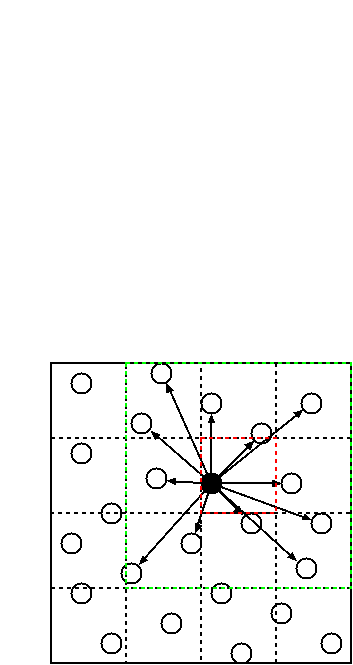
\includegraphics[width=\linewidth]{img/CellLists2.png}
    \caption{Finding the neighbours for the filled in particle $i$ by looking through all neighbouring cells, including its own cell, for particles within the cutoff distance $H$}
    \label{fig:cellList}
    \end{figure}

    The cell list is implemented by using a four dimensional vector where the first three dimensions are for the x, y and z coordinates for the cells and the fourth dimension is for storing the particles belonging to the cell.
    The amount of cells are decided by dividing the scene into cells of length $H$.
    The particles are then assigned to a cell according to Equation ~\ref{eq:assignCell}.
    If the particle moves out of its cell it is then assigned to the new cell.

    \begin{equation} \label{eq:assignCell}
        sjdfkljsf
    \end{equation}

% Should be mentioned early since it is used in mostly of the algorithms
\subsection{Kernel}
    A kernel function is used to simulate how particle-particle interactions decrease with the distance between the current particle and its neighbours. In SPH simulations this is an approximation of the Gaussian kernel function. Different kernels have been tested in previous works i.e. the poly6 kernel, the spiky kernel and the cubic spline kernel. According to Bender et. al.~\cite{bender} the cubic spline kernel presented by Monaghan~\cite{monaghan} was used. The kernel is described by Equation~\ref{eq:kernel}, where $q(x)=\frac{\left \| x \right \|}{h}$, $x$ is the distance between the current particle and a neighbour particle and $h$ is the support radius for the kernel. Particles further away than the support radius will not affect the current particle.   

    \begin{equation} \label{eq:kernel}
        W_h(q(x)) =  \frac{1}{\pi h^3} \left\{\begin{matrix}
        1 - \frac{3}{2}q^2 + \frac{3}{4}q^3 & 0 \leqslant q < 1 \\ 
        \\
        \frac{1}{4}(2-q)^3 & 1 \leqslant q < 2\\ 
        \\
        0 & q \geqslant 2
      \end{matrix}\right.
    \end{equation}

    The algorithm does also require the kernel gradient. To reduce the computational effort and memory requirements Bender et. al.~\cite{bender} introduce a scalar function $g(q) = \frac{\partial W_h}{\partial q} \cdot \frac{1}{h \left \| x \right \|}$. The gradient kernel is then calculated by $\partial W_h(q(x)) = x \cdot g(x)$. The gradient kernel is described by Equation ~\ref{eq:gradKernel}. 

    \begin{equation} \label{eq:gradKernel}
        \partial W_h(q(x)) =  x \cdot \frac{1}{h \left \| x \right \|} \cdot \frac{1}{\pi h^3} \left\{\begin{matrix}
        - 3q + \frac{9}{4}q^2 & 0 \leqslant q < 1 \\ 
        \\
        - \frac{3}{4}(2-q)^2 & 1 \leqslant q < 2\\ 
        \\
        0 & q \geqslant 2
      \end{matrix}\right.
    \end{equation}
    % maybe specify x here as well 

    It is important to use the same kernel function for both $W_h$ and $\nabla W_h$ to get the prediction and the correction step to be compatible to each other. 


\subsection{Divergence solver}
\subsection{Density solver}

\subsection{Navier-stokes}
% Write about non pressure forces, velocity osv..?
\subsection{Adapted time step}

% CFL condition, explain why its necessary and how its assured that each rendered frame has the same time step.
In order to assure a stable simulation it is necessary to adapt the time step depending on the motion. 
The quicker the particles move the smaller time steps are taken such that the numerical 
error of the explicit time integration is negligible. For this is a condition proposed by Courant–Friedrichs–Lewy used often refered as the CFL-condition show in equation \ref{eq:cfl}. The time step $\Delta t$ is equal to a fraction of the particle's diameter $d$ divided by the maximum velocity $\vect{V_{max}}$ in the scene.

\begin{equation}\label{eq:cfl}
\Delta t \leq \frac{0.4 \cdot d}{\vect{V_{max}}}
\end{equation}

Each rendered frame however have a constant time step in order to ensure no speed change in the playback of the rendered video. This is decided from the user side as a desired fps parameter. This means that the simulation loop can iterate multiple times within each frame adaptively depending on the maximum velocity.

\subsection{Density and alpha factors}
\subsection{Screen space fluid rendering}

\section{Implementation}
%Details of how it was done
%What hardware
%What software
%Why did you do it that way?
%What limitations, if any, did this present?
%*No code*!!!!!
 
    % Talk about what we used for plugins, computers etc maybe or should this be in method?

\section{Results}
%What is the end product:
%What does it look like?
%How does one control and interact with it?
%How quick is it?
%What limitations does it have?
%Be self-critical and honest about it - or I will be



\section{Conclusions and Future Work}
%Based on the results and evaluation
%Say what you’ve done right... ...and what you’ve done wrong! - be honest!
%Suggest some possible ways that the work could have been done better
%Suggest some ways that it could be extended and improved by adding more effort

% Use ghost-SPH or similar

\bibliographystyle{ieeetr}
\bibliography{./refs}

\end{document}
